% !TeX spellcheck = de_DE

\subsection{Trainingsumgebung}
Im Folgenden soll der Aufbau der Trainingsumgebung beschrieben werden, welche es erlaubt verschiedenste Kreaturen ohne große Anpassungen zu trainieren. Die  Umgebung ist dabei aus den folgenden Klassen aufgebaut:

\begin{itemize}
	\item \texttt{DynamicEnviormentGenerator}
	\begin{itemize}
		\item \texttt{TerrainGenerator} %Todo change when replaced by package
		\item Verschiedenen Konfigurationsdateien
		\item \texttt{DebugScript}
	\end{itemize}
	\item allen anderen modifizierten ML-Agents Skripten
\end{itemize} 

In diesen Abschnitt wird nur auf den Aufbaue des \texttt{DynamicEnviormentGenerator} sowie dessen Hilfsklassen und nicht auf die ML-Agent-Skripte eingegangen. Die Hilfsklassen sind der \texttt{TerrainGenerator}, \texttt{GenericConfig} und dessen Implementierungen sowie das \texttt{DebugScript}. Erstere ist verantwortlich für die Generierung des Terrains, die Config-Dateien laden dynamisch die Einstellungen aus einer Datei und das letzte Skript beinhaltet hilfreiche Debug-Einstellungen. Die grundsätzliche Idee der Trainingsumgebung stammt von dem ML-Agents-Walker. Da an diesem keine Versuche mit Unterschiedlichen Umgebungen und Kreaturen durchgeführt wurden, ist der Aufbau des Projekts nicht dynamisch genug. 

\subsubsection{Dynamic Enviorment Generator}
Zur dynamischen Umsetzung der Trainingsarena werden alle Objekte zur Laufzeit erstellt. Die Generierung der Arena läuft dann wie folgt ab:
\begin{enumerate}
	\item Erstellen von $n$ Arenen, wobei $n$ eine zu setzende Variable ist. 
	\item Füge ein Ziel für die Kreatur in die Arena ein
	\item Generiere die Kreatur
\end{enumerate}

Die einzelnen (Teil)-Arenen bestehen aus einem Container-Objekt unter dem ein Terrain und vier Wall-Prefabs angeordnet sind. Diese Prefabs und weitere Elemente wie Texturen werden dynamisch aus einem Ressourcen-Ordner geladen, damit möglichst wenige zusätzliche Konfigurationen den Editor verkomplizieren. Das Terrain wird mit leeren Terraindaten vorinitialisiert und später befüllt. Hierbei kann die Position des Container-Objects in der Szenen wie folgt berechnet werden:
\begin{align}
	\begin{pmatrix}
	\lceil \frac{\text{Anzahl der Arenen}}{\sqrt{\text{Anzahl der Arenen}}} \rceil \\
	0 \\
	\text{Anzahl der Arenen} \mod \sqrt{\text{Anzahl der Arenen}} \\
	\end{pmatrix}
	 = 	\begin{pmatrix}
	 x  \\
	 y \\
	 z  \\
	 \end{pmatrix}
\end{align}
Alle anderen Objektpositionen müssen danach neu im lokalen Koordinatensystem gesetzt werden. Da die Unity-Standard-Texturen sehr hell sind sind, werden die Texturen bei der Initialisierung mit ML-Agents-Texturen, welche dunkler sind, getauscht. An das Terrain werden zuletzt Collider und ein \texttt{TerrainGenerator}-Skript angefügt. 

In Schritt 2. der Arenagenerierung muss beachtet werden, dass nach dem Erstellen des Zielobjekts das \texttt{WalkTargetScript} hinzugefügt wird. Am Ende des Erstellungsprozesses wird der Walker erstellt. Hierzu wird ein von den Creature-Generator-Team bereitgestelltes Paket\footnote{https://github.com/PG649-3D-RPG/Creature-Generation} benutzt. Das Paket stellt ein Klasse bereit, welche mit zwei Skript-Objekte konfiguriert wird. Zusätzlich wird ein seed übergeben, welcher reproduzierbare Kreaturen erlaubt. Die erstelle Kreatur muss danach mit den entsprechenden ML-Agent-Skripten versehen werden. Hierzu wird ein \texttt{WalkerAgent} Objekt als String übergeben. Dies ermöglicht es, mehrere unterschiedliche Agent-Skripte durch eine Änderung im Editor zu setzen. Somit können Reward-Funktion und Observation für zwei unterschiedliche Trainingsversuche getrennt, in eigenen Dateien, entwickelt werden.
\begin{figure}
	\centering
	\includegraphics[width=0.7\linewidth]{example-image-a}
	\caption[Konfigurationsmöglichkeiten des \texttt{DynamicEnviormentGenerator}]{Konfigurationsmöglichkeiten des \texttt{DynamicEnviormentGenerator} im Unity-Editor.} %TODO setz pictures
	\label{bspDEGOptionen}
\end{figure}

\begin{figure}
	\centering
	\includegraphics[width=0.7\linewidth]{example-image-a}
	\caption[Beispiel der generierten Trainingsumgebung]{Ein Beispiel der generierten Trainingsumgebung mit mehreren Arenen.} %TODO setz pictures
	\label{bspArena}
\end{figure}

\subsubsection{TerrainGenerator}
Da ein typisches Spieleterrain im Gegensatz zum ML-Agents-Walker-Terrain nicht flach ist, wurde ein neues Objekt erstellt, welches sowohl die Generierung von Hindernissen, als auch eines unebenen Bodens erlaubt. Um ein möglichst natürlich erscheinendes Terrain zu erzeugen wird ein Perlin-Noise verwendet. Dieses spiegelt jeweils die Höhe des Terrains an einen spezifischen Punkt wider. Im späteren Projektverlauf wurde dieses Skript durch den Terraingenerator des dazugehörigen Teams ersetzt.

\subsubsection{Konfigurationsobjekte}
Da sich die statische Konfiguration des ML-Agents-Walker als problematisch erwies, wurde die Konfiguration über die Laufzeit des Projekts dynamischer gestaltet. Zuerst wurden alle Konfigurationen im \texttt{DynamicEnviormentGenerator} gespeichert. Was unübersichtlich war und zu ständigen neubauen des Projektes führte. Deshalb wurde eine \texttt{GenericConfig} Klasse eingeführt, welche die im Editor eingestellten Optionen für die einzelnen Teilbereiche Terrain, Arena und ML-Agent in Json-Format in den Streaming-Asset-Ordner speichert. Da dieser Ordner beim bauen des Projekts in das fertige Spiel übertragen wird, sind diese Konfigurationen automatisiert dort vorhanden. 

Im Fall, dass das Spiel ohne Editor gestartet wird, was meist beim Training der Fall ist, lädt das generische Objekt aus den Json-Dateien die Einstellungen und ersetzt die Editorkonfiguration damit. Hierdurch ist ein ändern der Konfiguration des Spiels ohne neu-erstellen der Binärdateien ermöglicht. Diese Konfigurationsart fügt Abhängigkeiten zu dem Unity eigenen JsonUtility\footnote{https://docs.unity3d.com/ScriptReference/JsonUtility.html} hinzu.

\subsection{Erweiterung der Agent-Klasse}
\todo{texttt im Titel?}

\begin{figure}
	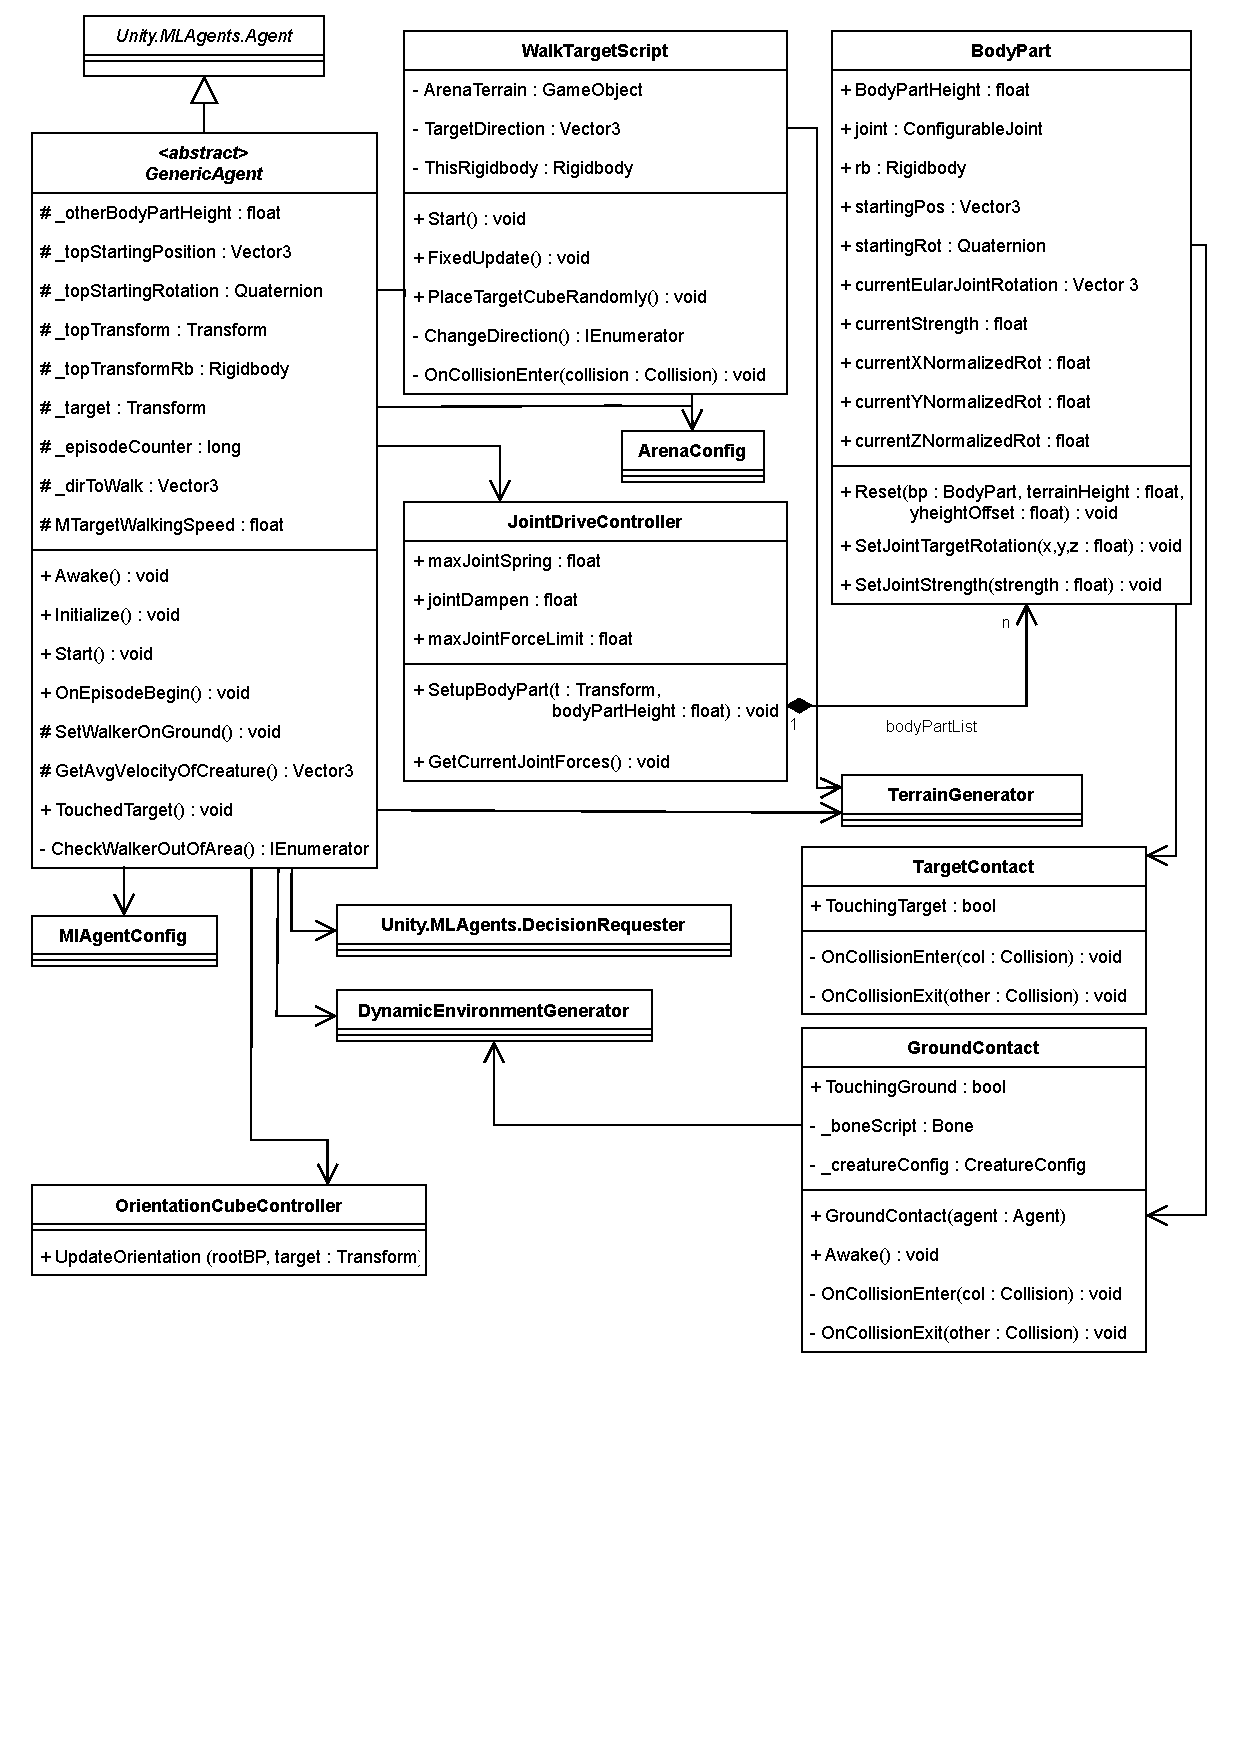
\includegraphics[width=\textwidth, trim={0cm 6.5cm 0cm 0cm}, clip]{resources/img/PG_Agent.drawio.pdf}
	\caption{UML-Diagram der GenericAgent-Klasse und weitere relevante Klassen}
	\label{fig:umlAgent}
\end{figure}

Als eine Erweiterung der \texttt{Agent}-Klasse von ML-Agents stellt die \texttt{GenericAgent}-Klasse das Verbindungsst"uck zwischen dem ML-Framework und der Unity-Engine dar. Im Folgenden wird der Aufbau der Klasse \texttt{GenericAgent} sowie derer Hilfsklassen \texttt{JointDrive\-Controller}, \texttt{BodyPart}, \texttt{OrientationCubeController} und \texttt{WalkTargetScript} erläutert und die Funktionalität dieser Klassen erklärt. Zur Veranschaulichung befindet sich in Abbildung \ref{fig:umlAgent} ein UML-Diagram. Der Aufbau dieser Klassen orientiert sich dabei sehr stark an die Implementierung des ML-Agents Walker.

\subsubsection{GenericAgent}

Die kontrollende Instanz einer konkreten Trainingsumgebung ist die \texttt{GenericAgent}-Klasse. Diese ist dazu in der Lage, mit dem Modell des ML-Frameworks zu interagieren, also sowohl Beobachtungen der Trainingsumgebung weiterzugeben also auch die Ausgaben des Modells anzunehmen (und zu verarbeiten). Außerdem ist die Klasse f"ur die Instandhaltung der Trainingsumgebung verantwortlich, indem sie Events der Umgebung verarbeitet (z.B. das Erreichen des Targets oder das Verlassen des zugänglichen Bereiches) und ggf. spezifizierte Routinen wie das Zur"ucksetzen der Umgebung durf"uhrt.
Schließlich muss die \texttt{GenericAgent}-Klasse noch die Rewards f"ur die Trainingsumgebung verteilen. Zu diesem Zweck ist die Klasse als \textit{abstract} definiert, da diese Rewardfunktionen stark von der Aufgabe des Agents abhängig sind. So benötigt zum Beispiel ein Agent, welcher ein bestimmtest Ziel möglichst schnell erreichen soll eine andere Reward-Funktion als ein Agent, welcher sich möglichst gut vor dem Spieler verstecken soll. Verschiedene Agents können so ohne Redundanz einfach als eine Erweiterung der \texttt{GenericAgent}-Klasse implementiert werden.

\todo{Mehr auf Reward-Funktionen eingehen oder erst bei konkreten Agents?}

\subsubsection{JointDriveController und BodyPart}

Um die Ingame-Repräsentation (also die generierte Creature) des Agents zu kontrollieren, besitzt der \texttt{GenericAgent} einen \texttt{JointDriveController}. Bei der Initialisierung der Trainingsumgebung wrappt der \texttt{JointDriveController} die verschiedenen Unity-Transforms der Creature in Instanzen der Hilfsklasse \texttt{BodyPart}. Die Klasse \texttt{BodyPart} gibt uns leichten Zugang zu häufig benötigten Funktionalitäten, wie zum Beispiel das Zur"ucksetzen oder Steuern des Transform. Auch besitzt ein \texttt{BodyPart} n"utzliche Informationen "uber das jeweilige Transform, welche dem ML-Modell weitergegeben werden können. Nach der Initialisierung stellt der \texttt{JointDriveController} nur noch das Verbindungsst"uck zwischen der \texttt{GenericAgent}-Klasse und der verschiedenen \texttt{BodyPart}-Instanzen dar.


\subsubsection{OrientationCubeController}

Da sich das Target des Agenten potentiell "uberall innerhalb einer großen (und weitgehend unbekannten) Ingame-Umgebung befinden kann, ist es hilfreich, die gezielte Laufrichtung des Agenten an eine einheitliche Position zu platzieren. Hierf"ur besitzt jeder Agent einen sogenannten \textit{OrientationCube}, welcher an einer festen Position relativ zum Agenten steht und sich lediglich in die Richtung des Targets dreht. So kann der Agent (und infolgedessen das ML-Modell) einfach den OrientationCube referenzieren, um die Laufrichtung zu bestimmen. Der \texttt{OrientationCubeController} stellt daf"ur die Reorientierungsfunktion des OrientationCubes bereit.


\subsubsection{WalkTargetScript}

Größtenteils unabhängig vom Agenten agiert das Target mithilfe des \texttt{WalkTargetScript}. Die Hauptaufgabe des Scripts ist es, das Target zu steuern (sowohl Neuplatzierung bei einem Reset, als auch normale Bewegungen innerhalb einer Episode) und beim Eintreten eines CollisionEvents zwischen dem Target und dem Agenten den Agenten zu notifizieren. Da zurzeit das Target nur aus einer Kugel besteht, ist komplizierteres Verhalten nicht notwendig.


\subsection{NeroRL \& ML-Agents}
% Jannik

Für das Training der Kreaturen kommt das Python-basierte Machine Learning Framework neroRL zum Einsatz. Die Auswahl ist in Kapitel \ref{} beschrieben. neroRL verbindet sich mit der Unity-seitig implementierten ML-Agents API und implementiert den PPO Algorithmus (siehe Kapitel \ref{}) auf Basis von PyTorch. Kapitel \ref{} beschreibt für die technische Umsetzung relevante Probleme, die die ursprüngliche Version von neroRL mit sich bringt. In diesem Kapitel wird die technische Umsetzung der Veränderungen an neroRL beschrieben, durch die das Framework für unser Projekt einsetzbar ist.

\subsubsection{Kontinuierliche Aktionsräume}
In der ursprünglichen Version von neroRL werden ausschließlich diskrete und multi-diskrete Aktionsräume unterstützt. Unsere Kreaturen benötigen kontinuierliche Aktionen. Die Klasse \texttt{ContinuousActionPolicy} implementiert einen Head (Kopf) für das neuronale Netzwerk, der kontinuierliche Aktionen umsetzt. Für jede Aktion des zugrundeliegenden Aktionsraumes werden $\mu$ (der Mittelwert) und $\sigma$ (die Standardabweichung) gelernt. Daraus wird eine Normalverteilung generiert, aus der dann ein tatsächliches Aktionstupel gesamplet werden kann. Als Verteilung wird die \texttt{Normal} Implementierung einer Gaußschen Normalverteilung aus PyTorch verwendet.

\subsubsection{Multi-Agent Builds}
Abhängig von den verfügbaren Rechenressourcen lassen sich maximal ca. 16 Builds parallel ausführen (LiDo3 cgpu01 Knoten mit 2 Intel Xeon E5-2640v4 und 2 NVIDIA Tesla K40). Um mehr Daten parallel zu sammeln, haben wir neroRL so erweitert, dass in einem Build mehrere Umgebungen mit jeweils einem Agenten parallel laufen können. Die von neroRL verwendeten Buffer Systeme verwenden dafür die Dimensionen $[worker][agent][timestep][content]$. Über $[worker]$ und $[agent]$ werden alle Daten genau einem Agenten in einem der ausgeführten Builds zugeordnet. Für die $[timestep]$ Dimension wird außerdem für jeden Build und Agenten festgehalten, welches der aktuelle Zeitschritt ist. Da Umgebungen zu unterschiedlichen Zeitpunkten terminieren und zurückgesetzt werden, ist es möglich, dass die Zeitschritte zwischen verschiedenen Agenten nicht synchronisiert sind. Sobald genug Daten für die definierte Batchgröße gesampelt sind, werden diese von den verschiedenen Builds und Agenten eingesammelt und in einem Batch kombiniert, das dann an den Trainingsalgorithmus übergeben wird.

\subsubsection{Optimierung der Trainingsqualität}
Nach Fertigstellung der Implementierung der Unterstützung von kontinuierlichen Aktionen zeigen die ersten Trainingsergebnisse unzureichende Ergebnisse. Während das Training der ML-Agents Walker Beispielumgebung mit ML-Agents nach ca. 30 Millionen Schritten einen durchschnittlichen Reward von ca. 2000 erreicht, erreicht neroRL auch nach über 150 Millionen Schritten nur einen Reward von ca. 220. Eine qualitative visuelle Bewertung des gelernten Verhaltens zeigt, dass der Walker sich zwar gezielt auf die erste Position des Ziels zubewegt, allerdings nach dem Verschieben des Ziels nicht in der Lage ist, sich umzudrehen. 
Um die Qualität des Trainings mit neroRL zu steigern, werden verschiedene Optimierungen verwendet.

\begin{itemize}
	\item \textbf{Normalisierung der Observationen:} Die Observationen werden durch den Sampler automatisch normalisiert, um das Training zu stabiliseren und vor ausreißenden Werten zu schützen.
	\item \textbf{Squashing:} Grundsätzlich können die aus dem Netzwerk gesampleten kontinuierlichen Aktionen im Intervall $[-\infty;\infty]$ liegen. Auf Unity liegen die Aktionen im Intervall $[-1;1]$ und werden dementsprechend abgeschnitten. In einigen Fällen hat sich Tanh-Squashing als eine Methode erwiesen, um die Trainingsqualität mit kontinuierlichen Aktionen zu steigern und die Aktionen auf das Intervall $[-1;1]$ zu projizieren, anstatt diese abzuschneiden (vgl. \cite{}). Unsere Implementierung von Tanh-Squashing wurde jedoch verworfen, da diese konsistent das Exploding-Gradients-Problem ausgelöst hat und das Training somit fehlgeschlagen ist. 
\end{itemize}


\subsection{LiDO3}
% Nils
Wie bereits erwähnt, werden die Berechnungen jeweils auf den HPC der TU Dortmund ausgeführt. Um auf LiDO3 zu arbeiten wird mit Hilfe eines Gatewayservers auf das Cluster zugegriffen. Der Zugriff ist ausschließlich über das TU Dortmund Netzwerk möglich. Über den Gatewayserver kann ein Zugriff auf die Rechenressourcen direkt über die Shell oder über Skripte angefordert werden. Da die Shell-Methode einen dauerhaften Login erfordern würde, wird mit Skripten gearbeitet. Diese bestehen aus Konfigurationen für LiDO3 und den eigentlich Programmteil, welcher ausgeführt werden soll. LiDO3 nutzt als Jobmanager Slurm, weshalb die Skripte die Slurm-Syntax nutzen. Eine ausführliche Beschreibung die LiDO3 Konfiguration findet sich im Benutzerhandbuch\cite{lido};

% TODO hier Skript richtig einfügen
\label{prog:lidoSkript}
\begin{verbatim}
#!/bin/bash -l
#SBATCH -C cgpu01
#SBATCH -c 20
#SBATCH --mem=40G
#SBATCH --gres=gpu:2
#SBATCH --partition=long
#SBATCH --time=48:00:00
#SBATCH --job-name=pg_k40
#SBATCH --output=/work/USER/log/log_%A.log
#SBATCH --signal=B:SIGQUIT@120
#SBATCH --mail-user=OUR_MAIL@tu-dortmund.de
#SBATCH --mail-type=ALL
#-------------------------------------

GAME_NAME="GAME_NAME"
GAME_PATH="/work/USER/games/$GAME_NAME"


module purge
module load nvidia/cuda/11.1.1

source /work/USER/anaconda3/bin/activate
conda activate /work/mmarplei/grudelpg649/k40_env

chmod -R 771 $GAME_PATH
cd $GAME_PATH

srun mlagents-learn /work/smnidunk/games/config/Walker.yaml --run-id=$GAME_NAME --env=t.x86_64 --num-envs=6 --no-graphics

\end{verbatim}

In dem Beispielskript \ref{prog:lidoSkript} sind Anweisungen an die LiDO-Umgebung jeweils mit einem Kommentarzeichen gefolgt von \emph{SBATCH} gekennzeichnet. Die Konfiguration wird so gewählt, dass eine maximale Laufzeit mit exklusiven Ressourcenrechten auf den Rechenknoten besteht. Zusätzlich muss sichergestellt werden, dass eine Grafikkarte zur Verfügung steht. Diese stehen auf den \emph{cgpu01}-Rechenknoten mit jeweils 20 CPU-Kernen und 48 Gigabyte RAM zur Verfügung. Die maximale Laufzeit des Prozesses ist bei den GPU-Knoten auf \emph{long} begrenzt, was 48 Stunden entspricht. Es wird jeweils ein Log mitgeschrieben, aus dem der Trainingsfortschritt gelesen werden kann und bei besonderen Ereignissen eine Mail geschickt, um sofort benachrichtigt zu werden, falls der Job fertig ist oder fehlschlägt.

\subsubsection{Kompatibilitätsprobleme}
Um das beschriebene Skript auszuführen, muss auf LiDO3 eine ML-Agents-Umgebung installiert werden. Dabei handelt es sich um ein Python Umgebung, mit PyTorch und CUDA. In dem Slurm-Skript \ref{prog:lidoUmgebung} ist die Einrichtung einer funktionierenden Umgebung dargestellt. 

\label{prog:lidoUmgebung}
% TODO hier Skript richtig einfügen
\begin{verbatim}
// LIDO UMGEBUNGSVARIABLEN
module purge
module load nvidia/cuda/11.1.1

source <anaconda3-path>/bin/activate
conda activate <env_to_install>
conda install torchvision torchaudio cudatoolkit=11.1 -c pytorch
python -m pip install mlagents==0.29.0 --force-reinstall
python -m pip install /work/mmarplei/grudelpg649/torch-1.10.0a0+git3c15822-cp39-cp39-linux_x86_64.whl --no-deps --force-reinstall 
\end{verbatim}

Für die Python-Installation wurde auf Anaconda\footnote{https://www.anaconda.com/} zurückgegriffen. Die installierte Anaconda-Arbeitsumgebung kann für die folgenden Schritte genutzt werden, indem die Slurm-Skripte diese am Anfang laden. CUDA kann als Kernelmodul in verschiedenen Versionen geladen werden oder per Anaconda installiert werden.

Problematisch ist die Installation von PyTorch, da ab Version 1.5 die Installationsbinärdateien keine Unterstützung für die von LiDO3 genutzten NVIDIA Tesla K40 Grafikarten bietet. Es besteht die Möglichkeit PyTorch zu bauen um die Unterstürzung zu erhalten. Dies musste für unsere Arbeitsumgebung nicht gemacht werden, da die PG-Betreuer ein Paket mit einer für LiDO funktionierenden PyTorch-Version von einer vorherigen PG zur Verfügung stellen konnten. Wie in \ref{prog:lidoUmgebung} dargestellt müssen zuerst die Abhängigkeiten von PyTorch, dann ML-Agents und zuletzt die spezielle PyTorch Version installiert werden, da sonst die Abhängigkeiten Probleme bereiten.

